\section{System Overview}

Before the design of segway can begin, it has to be determined which subsystems are to be designed. In \autoref{fig:ext_seg_over}, the detailed block diagram of the system was presented. As most of the hardware for the segway is already provided, the project will primary focus on designing the controllers in the system. This limitation can be seen in \autoref{fig:system_overview_block}. Here, the blue blocks are subsystem that are to be designed, while the grey blocks are not designed.


\begin{figure}[H]
	\centering
	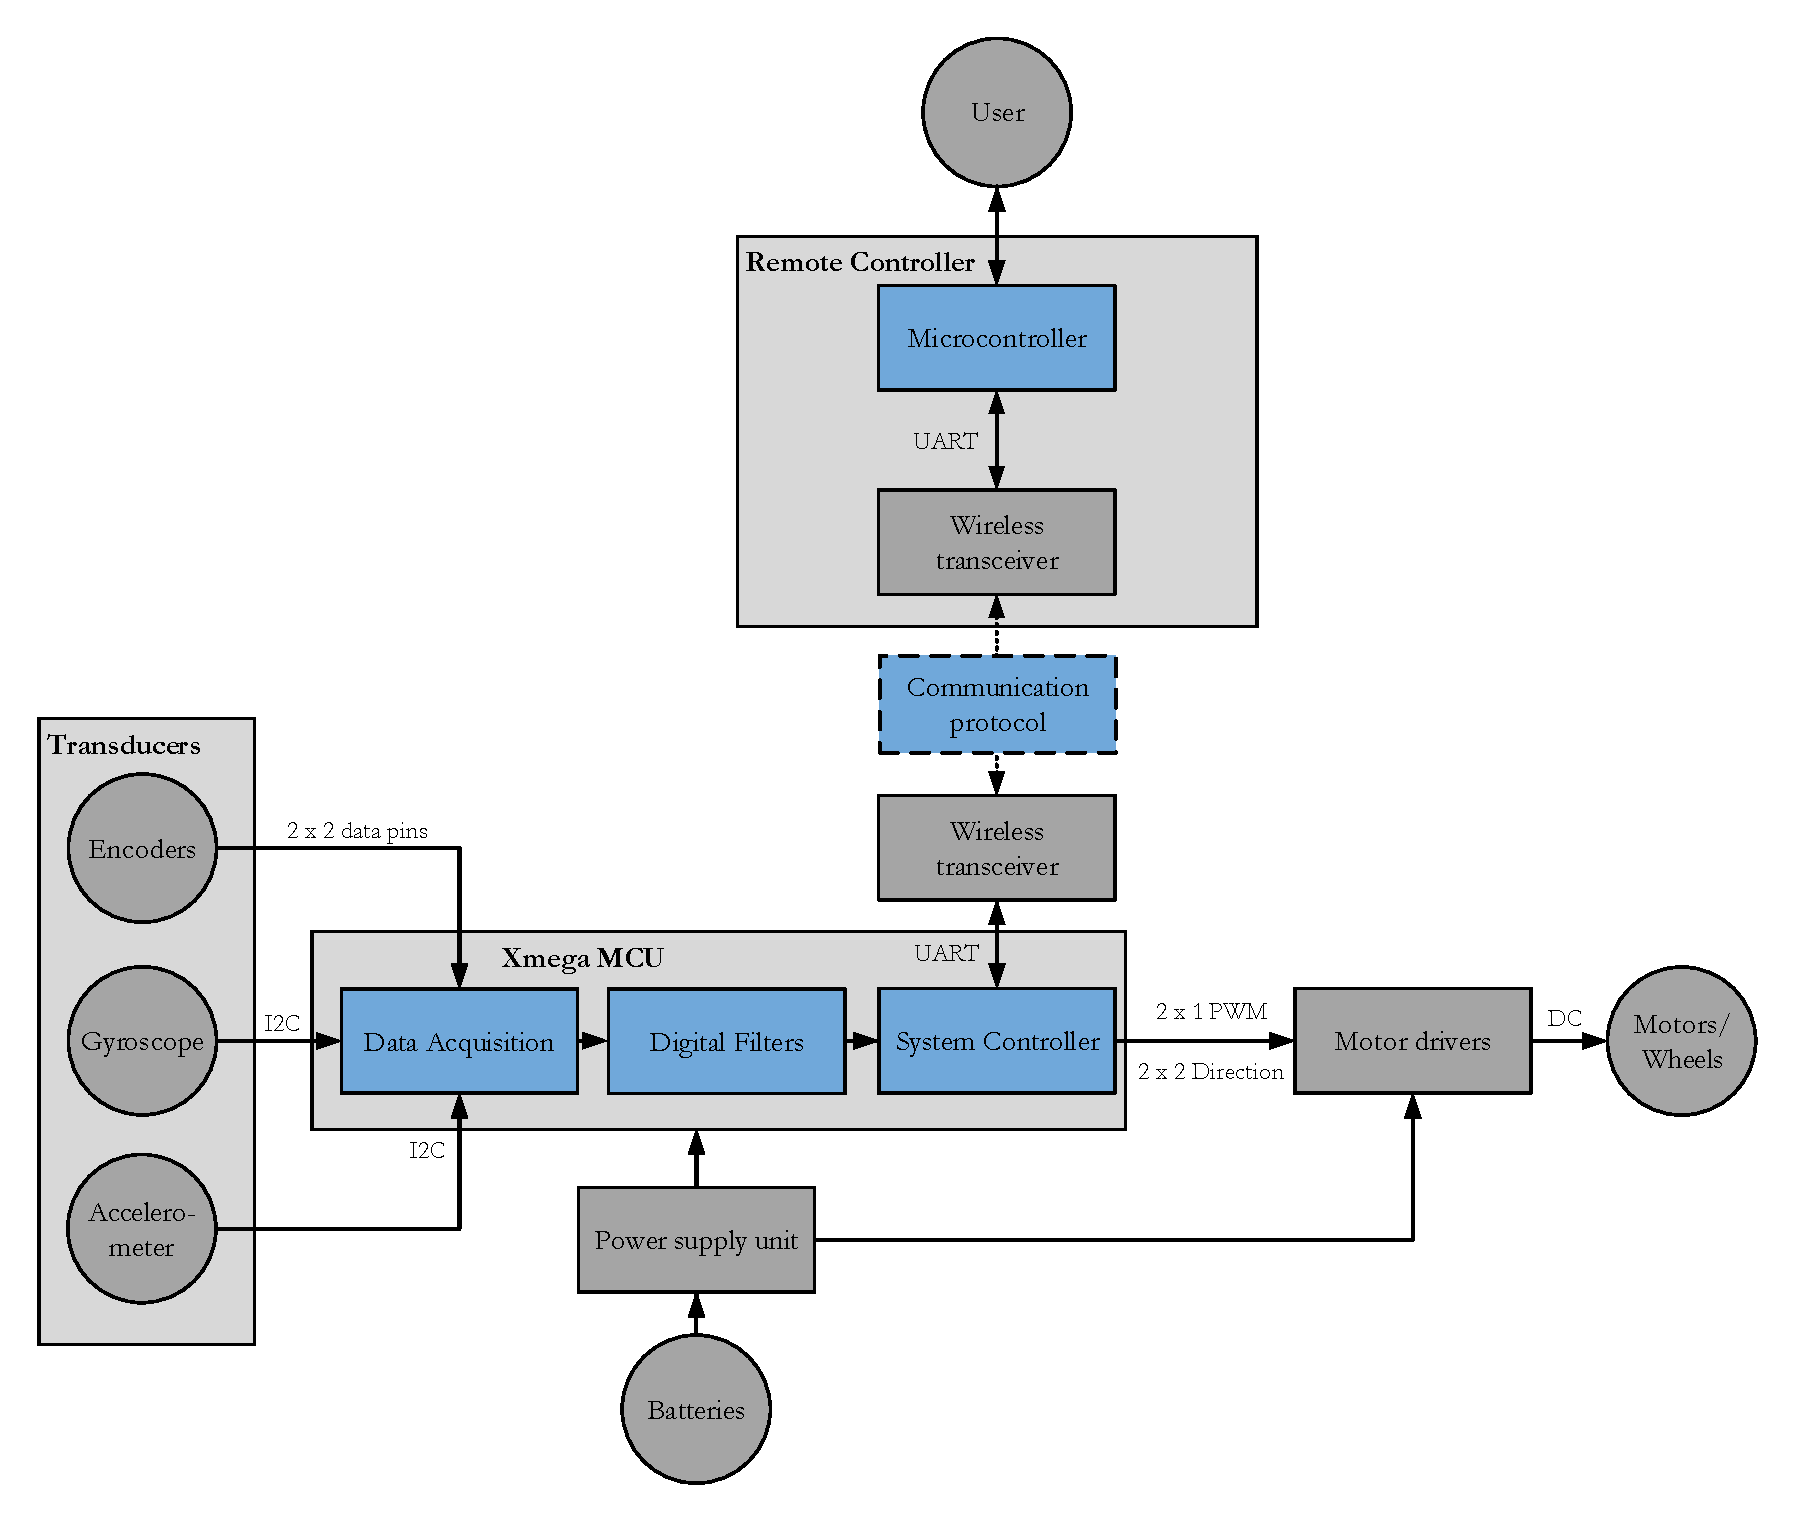
\includegraphics[width=0.95\textwidth]{design/figures/extendedOverviewGrayedWithInterfaces.pdf}
	\caption{Overview of the system. The blue blocks are blocks the design primary deals with.}
	\label{fig:system_overview_block}
\end{figure}
Note that a communication protocol has been inserted between the wireless transceivers. This is done because some "rules" has to be introduced in the communication between the remote controller and the MCU on the segway to ensure a proper data transfer without misunderstandings.

Also, a filter is inserted between the encoders and the MCU. To avoid breaking electrical interfaces and changing the electrical configuration of the segway, the filter is implemented as a digital filter, instead of an analog.

To ensure that subsystems can be designed parallel, the interfaces between subsystems have to be clarified. Data types transmitted between subsystems are shown in \autoref{fig:system_overview_block}. From left, the gyroscope and accelerometer transmits measured values through an $I^{2}C$ communication protocol, and the encoders data through two data pins. For external communication to the remote controller, data is transferred through a UART interface which is supported by both the wireless transceiver and the microcontroller. To control the motor drivers, a PWM signal is used for each motor, together with two direction pins.

\subsection{Control Loop Overview}\label{controlLoopOverview}
The system that controls the balancing of the segway can be described as a closed loop system, as shown in \autoref{fig:segOverview}. The segway is balanced through the use of three subsystems, namely the controller (D), the plant (G) and the sensors (H). It is assumed that the sensors are ideal, meaning that their frequency response is equal to unity i.e. $H(s) = 1$, as this block won't include any amplification or filtering, but solely measure. This is done since it is decided not to determine the sensor's transfer function, and that it will make the calculations easier by assuming that the measued output data is identical to the actual output. The input, R, is the desired angle of the segway, which for the balancing functionality, will be zero, i.e. the steady state upright position. The output $Y$ is the actual angle of the segway, denoted as $\theta_p$.

\begin{figure}[H]
\centering
\input{figures/modelBlockOverview.ralf}
\caption{A feedback loop of the system that controls the balance of the segway.}
\label{fig:segOverview}
\end{figure}

The plant is based on a model of the system that describes the movement of the segway, where the output is $Y = \theta_p$. This model is found in \autoref{ch:modelling}. %The input to the plant model is determined in \autoref{ch:modelling}, where the model is derived from an analysis of the segway. %The plant is used to directly change the output of the closed loop feedback system.

The controller block, D, generates the input to the plant, based on the difference between the desired angle, R, also known as the reference, and the actual angle measured by the sensor system, H. The output of the controller, U, is generated so that the error between output of the plant, Y, and the desired angle is minimized. The design of the controller unit is performed in \autoref{ch:Controller}.

%In the following chapter, the plant model is derived, as this lies the foundation for the controller design.

Now that the segway platform has been described, it is possible to set up the requirements for the system, which is done in the following chapter.



%The interface requirements is needed in order to determine the data type of the inputs and outputs of each subsystem.


%\section{Interface requirements} \todo{The section is still a sketch}
%\todo{reduce section}
%To ensure subsystems can be designed individually it is necessary to define the interface requirements. The interface requirements is needed in order to determine the data type of the inputs and outputs of each subsystem. 
%
%\subsection{Filter}
%
%The input of the filter is an analog signal from the encoders. The signal contains data about the rotation and direction of the motors. Since the inputs from the encoders are analog the best solution, are to make the filter analog as well. \todo{Is the encoder output analog or digital?}
%
%\subsection{Data Acquisition}
%
%As seen on \autoref{fig:system_overview_block} the data acquisition block receives input from the encoders, gyroscope, and accelerometer. Since the microcontroller only operates with digital signals any analog signal from the transducers has to be sampled into digital signal. 
%
%Another task is to convert measured data into understandable data types. This makes it easier to apply the measured data into control algorithm in the system controller.
%
%\subsection{System controller}
%
%Both data acquisition and the wireless transceiver transfers data to the system controller. The input from the data acquisition block is digital data from the transducers. Input from the wireless transceiver is digital as well but the communication protocol has to be the same as on both controllers.
%
%\subsection{Motor controller}
%
%The input of the motor controller is a digital signal from the system controller. The input could be data telling that the segway should move forward. Since the output of the motor controller is connected to the motor driver, it is necessary to insure that data from the motor controller is the same type of the motor driver.
%
%\subsection{Microcontroller for remote controller}
%
%
%
%\subsection{Communication protocol}
%
%
%
%\subsection{User input}
%
%
%
%
%\begin{enumerate}
%\item Modelling
%\item Designing subsystems
%\item System integration
%\item System implementation
%\end{enumerate}




